\setAuthor{Tundmatu autor}
\setRound{lõppvoor}
\setYear{2004}
\setNumber{G 2}
\setDifficulty{1}
\setTopic{Teema}

\prob{Veepark}
Veepargis on punane ja roheline liumägi. Joonisel on näidatud nende profiilid. Mari alustab punaselt liumäelt laskumist algkiiruseta, Juri aga lasküb roheliselt mäelt algkiirusega $v_0 = \SI{1}{m/s}$. Kumma kiirus on laskumise lõpuks suurem ja mitu korda, kui Jüri kaalub $m_j = \SI{70}{kg}$ ja Mari $m_m = \SI{60}{kg}$? Võib eeldada, et laskumise ajal mõjub neile mõlemale konstantne takistusjõud $F = \SI{20}{N}$.
\begin{center}
	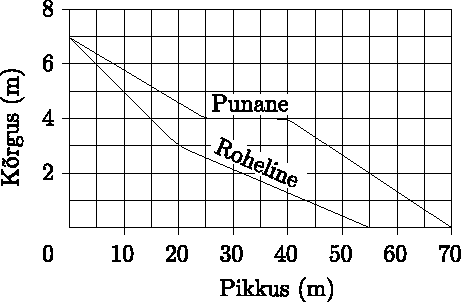
\includegraphics[width=0.7\linewidth]{2004-v3g-02-yl.pdf}
\end{center}

\hint

\solu
Nii Jüri kui ka Mari puhul peab kehtima energia jäävuse seadus:
$$
\frac{1}{2} m v_{0}+m g h=\frac{1}{2} m v+F s,
$$
kus $v_{0}$ on algkiirus, $h-$ mäe korgus, $v$ - lõppkiirus ja $F s-$ töö takistusjõu vastu. Avaldis lõppkiiruse jaoks saab kuju
$$
v=\sqrt{v_{0}^{2}+2 g h-2 F s / m}.
$$
Jooniselt leiame, et $h=\SI{7}{m}$. $s$ määramiseks leiame teepikkuse iga sirge lõigu jaoks ning liidame kokku. Jüri läbis teepikkuse
$$
s_{j}=\sqrt{20^{2}+4^{2}}+\sqrt{35^{2}+3^{2}}=\SI{55,5}{m}
$$
ning Mari teepikkus oli
$$
s_{m}=\sqrt{25^{2}+3^{2}}+15+\sqrt{30^{2}+4^{2}}=\SI{70,4}{m}
$$
Lõppkiiruse väärtuseks saame nüüd Mari jaoks
$$
v_{m}=\sqrt{0+2 \cdot 9,8 \cdot 7-\frac{2 \cdot 20 \cdot \num{70,4}}{60}} \approx \SI{9,5}{m/s}
$$
ning Jüri jaoks
$$
v_{j}=\sqrt{1+2 \cdot 9,8 \cdot 7-\frac{2 \cdot 20 \cdot \num{55,5}}{70}} \approx \SI{10,3}{m/s}
$$
Seega Jüri on lõpus \num{1,08} korda kiirem kui Mari.

\probend